\chapter{Object-based Analysis}

\section{HRV cloud objects}
The derivation of cloud objects as described in Sec. \ref{sec:cloud} yielded a total of \num{1107} HRV cloud objects for the five case days, with \SI{80}{\percent} single cell objects and \SI{20}{\percent} complex objects, which are multi cell objects with a number of splits and merges. The vast majority of the single cell objects has only a rather short life time of \SIrange{15}{30}{\minute}, with a median life time of \SI{30}{\minute} (Fig.~\ref{fig:cell_ltime}). As \remove[HD]{it} can been seen in Fig.~\ref{fig:cell_ltime}, the life time distribution \change[HD]{of}{for} the complex objects is broader \change[SL]{then}{than} the one for the single cells \change[HD]{. As to be expected,}{and} the complex objects \remove{also} have a longer life time with a median of \SI{60}{\minute}. There are no complex objects with a life time \remove{of} lower than \SI{30}{\minute} \remove[HD]{. This is} due to the definition of the complex objects. \remove[HD]{There are} At least two time steps \add[HD]{are} needed to develop splits or merges, so that the minimum life time of these objects is at least \SI{30}{\minute}. The multi-cell objects can be quite complex, with up to \num{26} splits or merges in one object (Fig.~\ref{fig:splits_merges}). \change[HD]{Those}{Such} objects \add[HD]{typically}represent large compact cloud fields which usually are present for a longer time \remove[HD]{range}. But most complex objects have only have very few splits or merges, with a median value of one split or merge. These objects \add[HD]{mainly} represent smaller cloud objects, which grow together to form larger objects. Splits and merges are roughly \change[HD]{similar}{similarly} abundant, but splits are a bit more frequent in the objects than merges. One reason for this is that the rather large and long living cloud fields tend \add[HD]{to} dissolve on the boundaries and \remove[HD]{so} create smaller objects that \add[HD]{do} not merge again.

Separating the complex objects at the split and merge points, and only conserving the objects prior to these points, an additional number of \num{2915} single cells can be derived. The life time distribution of the single objects derived from the complex objects is quite similar to the distribution of the single cell objects (Fig.~\ref{fig:single_cell}).

When only taking into account all single cells with a life time of at least \SI{30}{\minute}, to be consistent with the ground truth definition, the number of eligible objects decreases to \num{1584} objects. \change[HD]{But, as}{Additionally,} not all the validation area is covered by the radars, \add[HD]{and} only the objects inside the radar-covered area can be used for the validation. This reduces the number of eligible objects \add[HD]{further} to 1180. The \change[HD]{further}{subsequent} analysis was conducted with these objects.

\begin{figure}[htbp]
\centering
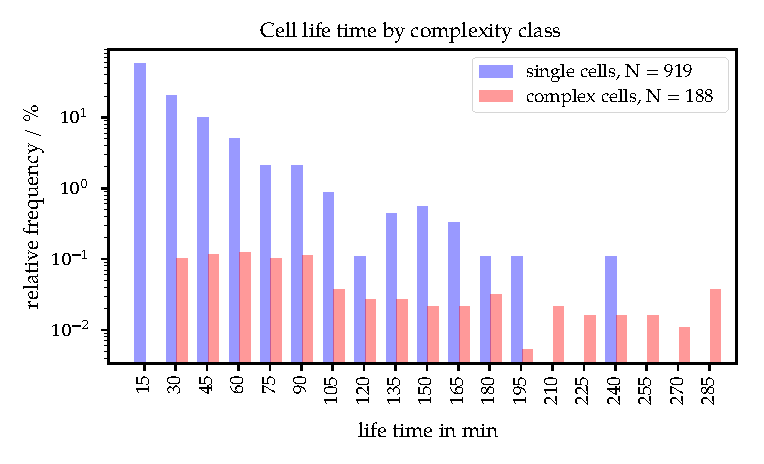
\includegraphics[width=\textwidth]{Grafiken/Abbildungen/cellclass_lifetime.pdf}
\caption{Comparison of the life time of single (blue) and multi cell (complex) objects (red).}
\label{fig:cell_ltime}
\end{figure}

\begin{figure}[htbp]
\centering
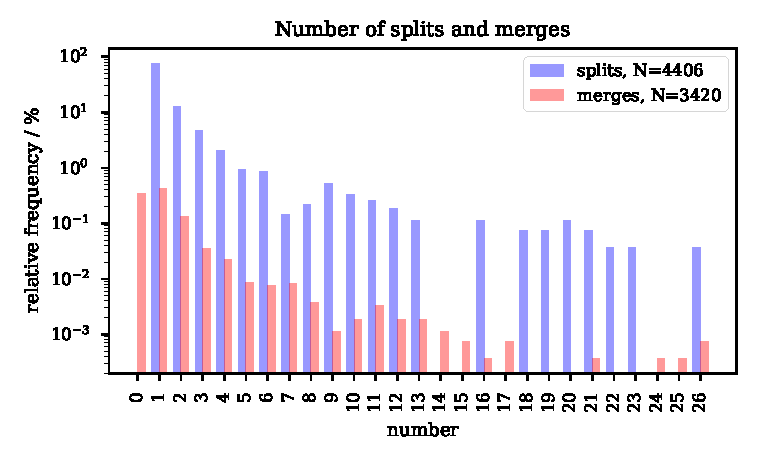
\includegraphics[width=\textwidth]{Grafiken/Abbildungen/splits_merges.pdf}
\caption{Distribution of number of splits and merges in the complex objects.}
\label{fig:splits_merges}
\end{figure}

\begin{figure}[htbp]
\centering
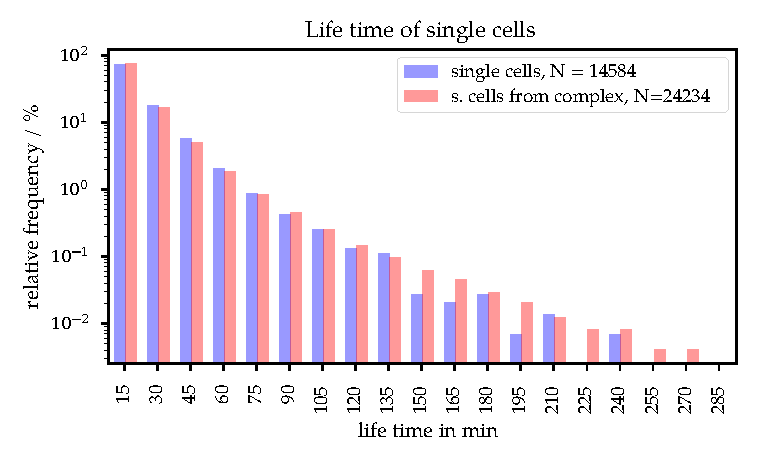
\includegraphics[width=\textwidth]{Grafiken/Abbildungen/single_from_complex_lifetime.pdf}
\caption{Comparison of the life time of single cell objects (blue) and the single cell objects derived from complex objects (red).}
\label{fig:single_cell}
\end{figure}

\section{Ground truth objects}
Using the weather radar data and applying the approach presented in Sec. \ref{sec:haci}, \num{526} ground truth objects with a minimum life time of \SI{30}{\minute} could be derived in the time frame 05:00 am UTC to 05:00 pm UTC for the six case days. This \add[HD]{number} is only around \SI{53}{\percent} of the number of cloud objects, \remove[HD]{but to be expected} as not all clouds form precipitation. 

As it can be seen in Fig. \ref{fig:haci_frequency}, the proportion of the number of ground truth objects is quite variable for the case days. Most of the ground truth objects stem from the three case days 3\textsuperscript{rd} July 2010, 23\textsuperscript{rd} May 2012 and 20\textsuperscript{th} July 2013, which account for more then \SI{80}{\percent} of all ground truth objects. 

As is also visible from Fig. \ref{fig:haci_frequency}, the \change[HD]{rate}{ratio} of ground truth objects matching with at least one cloud object is almost or equal to \SI{100}{\percent} for \remove[HD]{the} most case days. The only exception is 28\textsuperscript{th} June 2010 where the \change[HD]{rate is only}{ratio lies} a bit above \SI{60}{\percent}. This day is also the day with the highest percentage of cloud objects, with around \SI{30}{\percent} of all cloud objects having been derived from this day. On this case day, there is convective development over \change[HD]{the largest part}{large parts} of Germany with the exception of the \change[]{north east}{North-East}. Most of the convective developments are rather isolated, leading to the rather high percentage of cloud objects coming from this day. But \remove{the} most of these cells do not form precipitation. Convective cells forming precipitation start to develop along and downstream of the Black Forest in South West Germany and the Vosges Mountains in Eastern France. But these cells \change[SL]{have are}{exhibit} rather complex developments and thus are missed by our cloud object derivation approach. \remove{But} For the other case days, our cloud object approach works quite well and \change[HD]{gets}{captures} the most \change[HD]{interesting}{prominent} developments.

\begin{figure}[htbp]
\centering
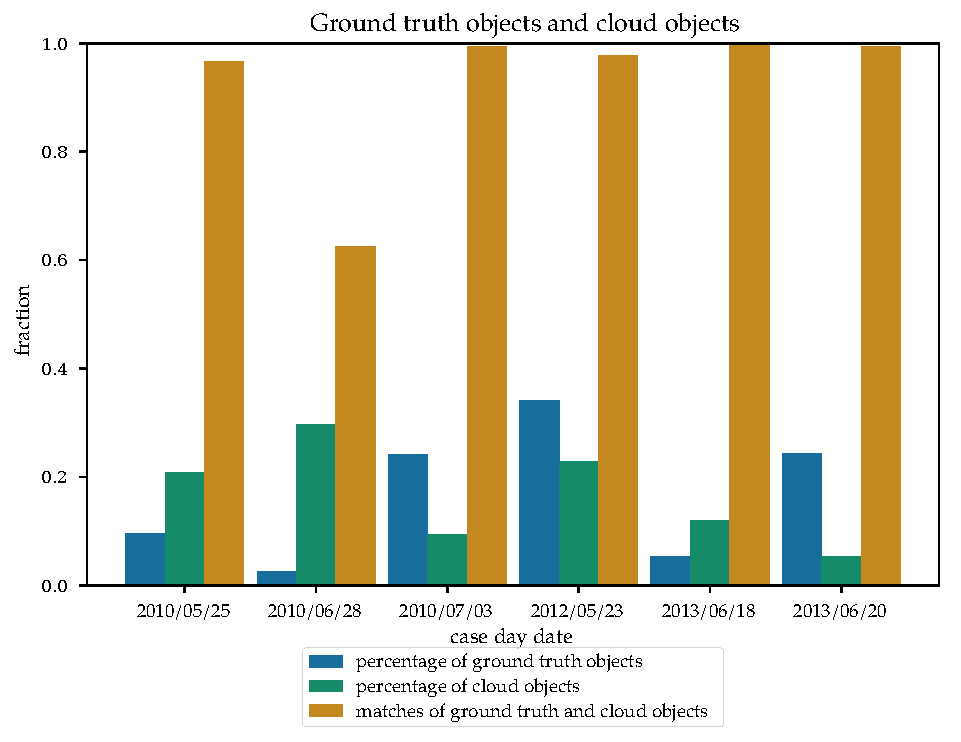
\includegraphics[width=\textwidth]{Grafiken/Abbildungen/haci_hrv_frequencies.pdf}
\caption{Proportion ground truth objects of the case days to the total number of ground truth objects (blue), proportion of cloud objects to total number of cloud objects, (green) and proportion of ground truth objects matching with cloud objects (yellow).}
\label{fig:haci_frequency}
\end{figure}

\section{Validation results}
The validation of the \SI{30}{\minute} forecast of the NWC\,SAF CI product \change[SL]{v2016}{v2018} using the approach presented above yields the \change[HD]{result}{validation statistics} given in Fig.~\ref{fig:validation_result1} and Tab.~\ref{tab:validation_result}. Although the number of cases used for the validation seems \change[HD]{sufficient enough}{sufficiently large}, only two of the CI probability levels can be evaluated, as there are only true positive cases for the levels \SIrange{25}{50}{\percent} and \SIrange{75}{100}{\percent}. For all CI probability levels, the vast majority of cases are true negative cases. True positives, false positive and false negative seem to be quite randomly and unequally distributed over the CI probability levels. The total number of true positive cases sums up to only 15 cases, with ten for level \SIrange{25}{50}{\percent} and five for level \SIrange{75}{100}{\percent}. So the validation results are statistically not very robust and need to be \change[HD]{taken into account}{interpreted} cautiously. 

\begin{table}[htb]
\centering
\caption{Confusion matrix for the validation result}
\begin{tabular}{cccc} 
\toprule
\multirow{2}{*}{CI product detection} &     & \multicolumn{2}{c}{weather radar detection} \\
							   						  \cmidrule{3-4}
									  &     &  yes & no \\
\midrule
\multirow{2}{*}{level 1}  & yes &    0 &    1 \\
	                                  & no  &   14 & 1157 \\ 
\midrule
\multirow{2}{*}{level 2}  & yes &   10 &   31 \\ 
	                                  & no  &    9 & 1125 \\ 
\midrule	                                  
\multirow{2}{*}{level 3}  & yes &    0 &    2 \\ 
	                                  & no  &   14 & 1156 \\ 
\midrule	                                  
\multirow{2}{*}{level 4}  & yes &    5 &    5 \\ 
	                                  & no  &   13 & 1152 \\
\addlinespace
\bottomrule
\end{tabular}
\label{tab:validation_result}
\end{table}

One reason for this is, that, as shown in Section~\ref{sec:diurnal_cycle} co-occurences of CI detections with radar reflectivity factors of more or equal to \SI{35}{dBZ} are quite rare. Thus, our validation approach of using objects based on a radar reflectivity factor of \SI{35}{dBZ} is rather strict \change{. But this}{and} ensures that the rate of false detections is not increased artificially.

As visible in Fig.~\ref{fig:validation_result2}a, the two levels for which true positives are existing behave quite differently in terms of POD and FAR. The lower CI probability level has a rather high POD of \num{0.52} but also a quite high FAR of \num{0.76}. As to be expected, the higher CI probability level exhibits a lower POD of a  \num{0.28} but also a lower FAR of \change[SL]{0.54}{0.50}.

%Taking into account the distribution of the CI detections over the case days (Fig.~\ref{fig:validation_case_days}), it has to be noted that the contribution of the different case days to the validation result is quite different. So, the most true positives come from the 23\textsuperscript{rd} May 2012 while there are no true positives on 28\textsuperscript{th} June 2010. In fact the distribution of true positives for the case days looks quite similar to the distribution of ground truth objects in Fig.~\ref{fig:haci_frequency}} and the distribution of false positives looks quite similar to the distribution of cloud objects. So the result of the study is probably influenced by the number of available objects to be evaluated and thus the validation  is statistically not very robust. A higher number of case days could probably eliminate this behaviour. Moreover, there are no false negatives for the first three case days while the second three case days have them. This can be an indication that the algorithm of the NWC\,SAF CI product works better for certain weather patterns than for others. On the first three case days the convective development started over over France or the border region between France and Germany and than moved inside the study area. On the second three case days the convective development started within the study area. So, differences in meteorological and also geographical conditions can be causes for this different behaviour in the false negative cases. But, as the NWC\,SAF product has been mainly tuned over France, there is also the possibility that the algorithm parameters work best over France and have to be re-calibrated for different regions and different meteorological conditions. This should be investigated further in future studies concerning the NWC\,SAF CI product.

\add[SL]{Taking into account the number of CI detections for the case days} (Fig.~\ref{fig:validation_case_days}), \add[SL]{it has to be noted that the contribution of the different case days to the validation result is quite different. Most true positives come from the 23\textsuperscript{rd} May 2012, while there are no true positives on 28\textsuperscript{th} June 2010. In fact the distribution of true positives for the case days looks quite similar to the distribution of ground truth objects in} Fig.~\ref{fig:haci_frequency} \add[SL]{and the distribution of false positives looks quite similar to the distribution of cloud objects. So the result of the study is probably influenced by the number of available objects to be evaluated and thus the validation  is statistically not very robust. A higher number of case days could probably help to address this behaviour. Moreover, there are no false negatives for the first three case days in contrast to the second three case days. This can be an indication that the algorithm of the NWC\,SAF CI product works better for certain weather patterns than for others. On the first three case days, the convective development started over France and the border region between France and Germany, and then moved inside the study area. On the second three case days, the convective development started within the study area. So, differences in meteorological and geographical conditions could be causes for this different behaviour. But as the NWC\,SAF product has been mainly tuned over France, there is also the possibility that the algorithm parameters work best over France and have to be re-calibrated for different regions and different meteorological conditions. This aspect should be investigated further in future studies}

Considering \add{the} CSI (Fig.~\ref{fig:validation_result2}b) the two CI probability categories \remove{are are}{lie} in the same range, with a \change[HD]{CSI}{value} of \num{0.19} for \SIrange{25}{50}{\percent} CI probability, and \num{0.21} for \SIrange{75}{100}{\percent} CI probability. This means that only around one fifth of really occuring events \change[HD]{where}{were correctly} forecast \remove[HD]{correctly}, with the higher CI probability \change[HD]{having a bit higher skill to forecast an event correctly}{showing a slightly higher skill}. 

For the HSS the picture looks similar. The higher CI probability category \add[HD]{again} has a higher prediction skill, with an HSS value of \num{0.31}, whereas the lower CI probability category has an HSS of \num{0.34}. \remove{But as} Both values \change[HD]{are}{lie} above 0, \change[HD]{both categories have the}{indicating a} skill to forecast an event better than chance. Also, both HSS values are higher than the CSI values, implying that the strength of the forecast is more on the side of correctly \change[HD]{not forecasting an non-event}{predicting true negatives}, which is not taken into account in the CSI.


\begin{figure}[htbp]
\centering
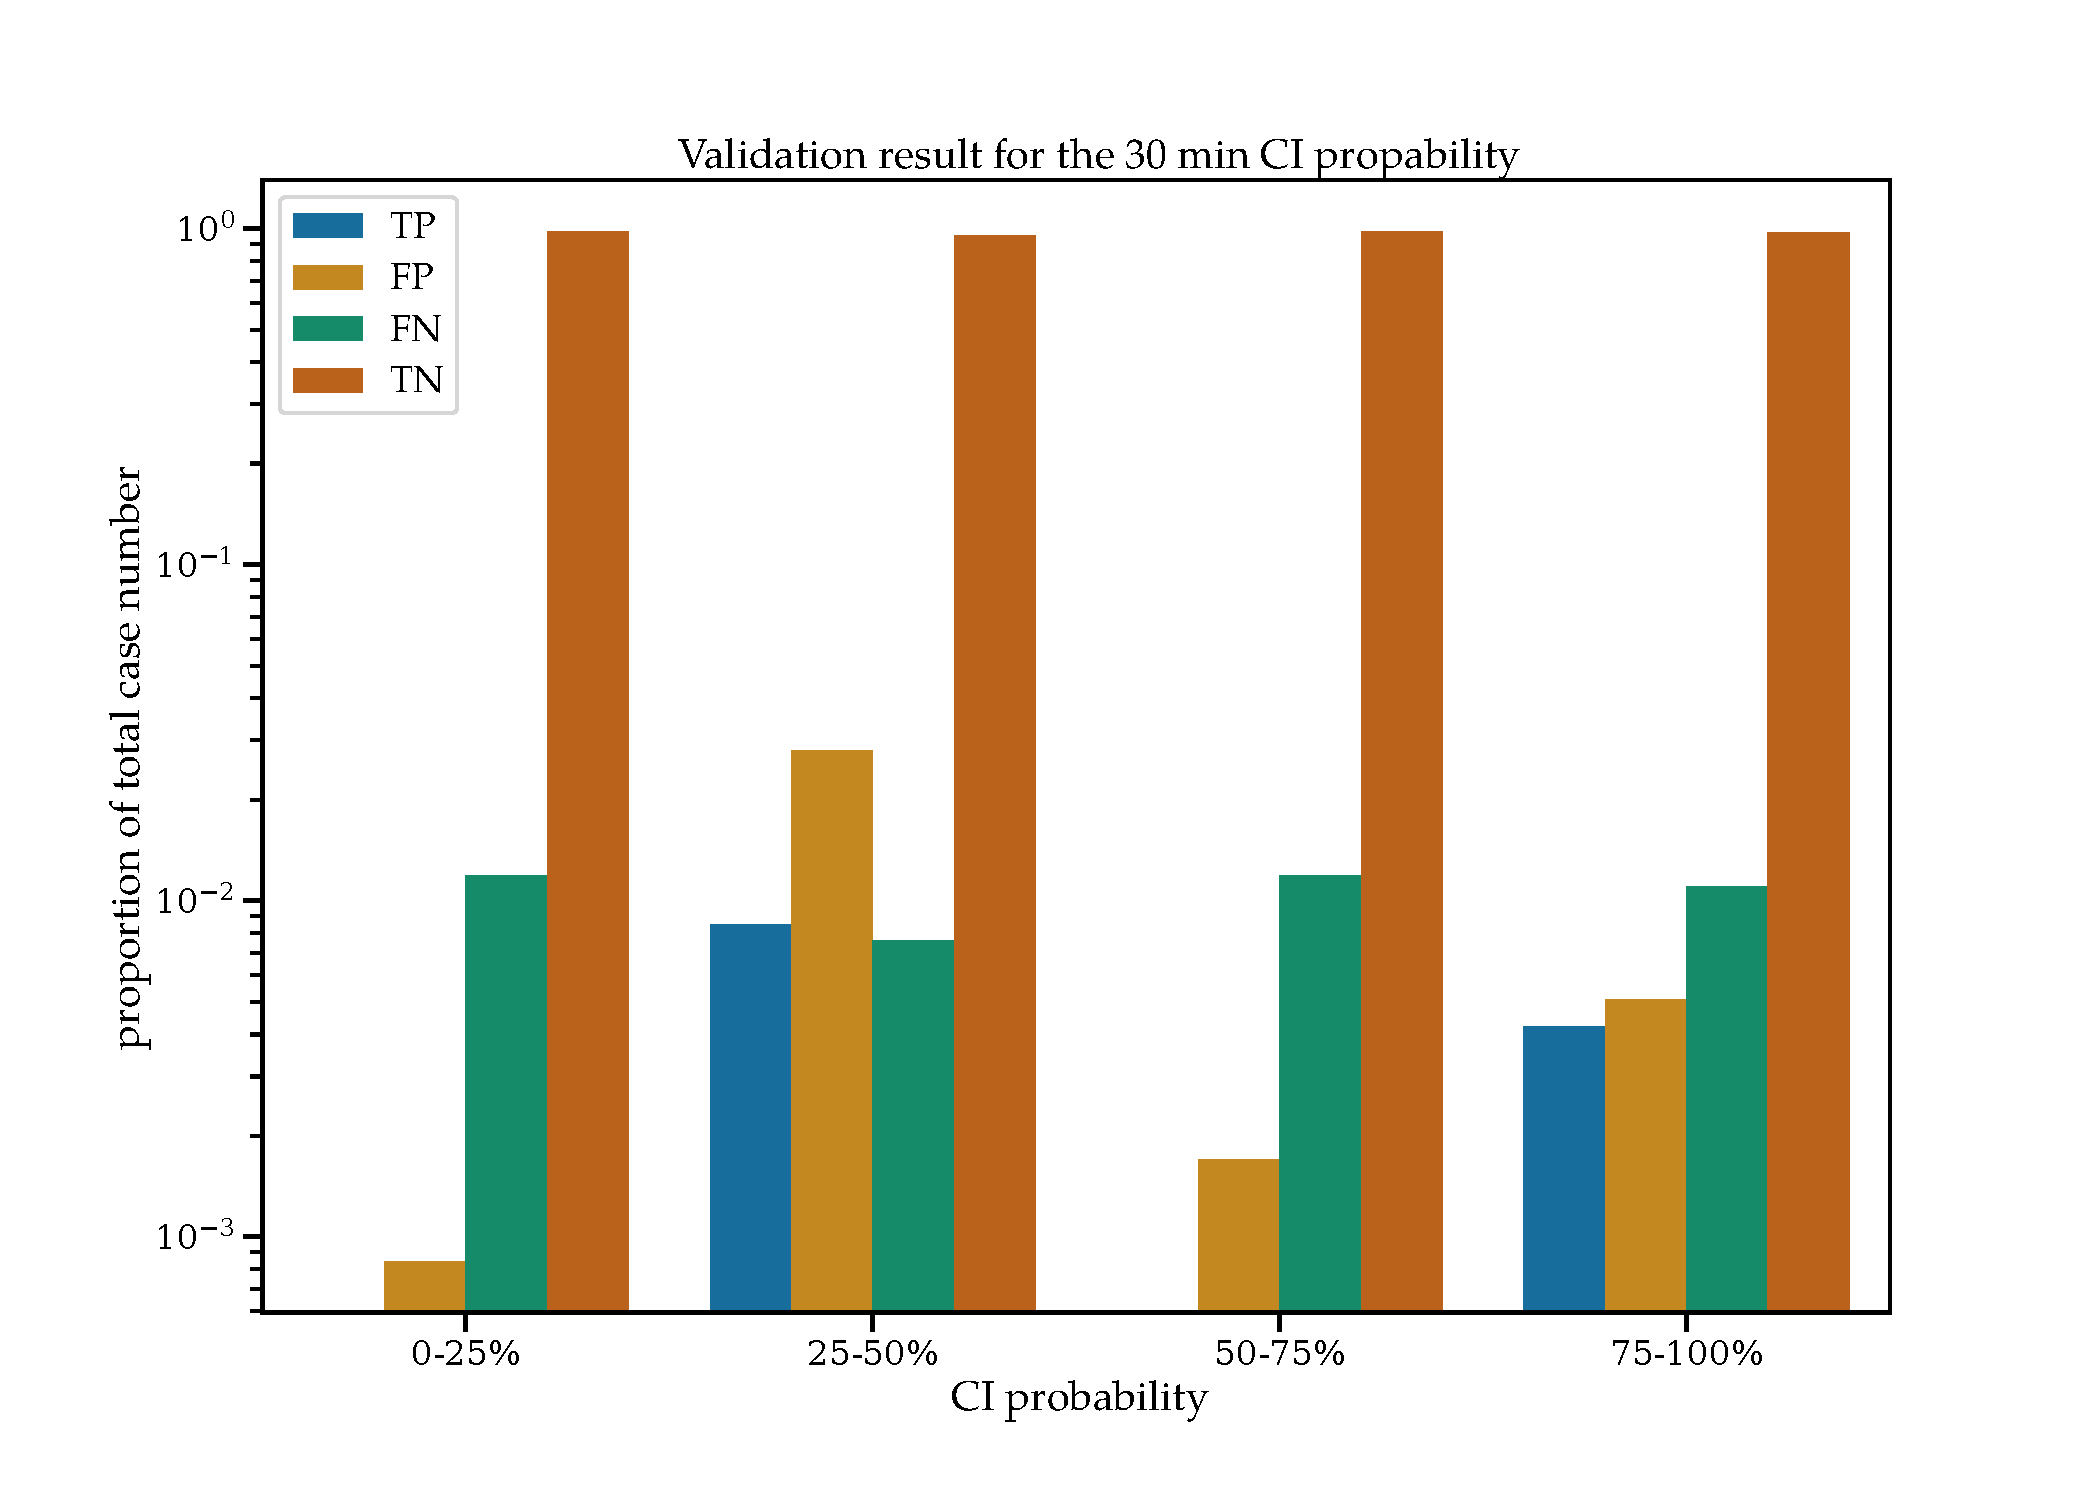
\includegraphics[width=0.8\textwidth]{Grafiken/Abbildungen/validation_plot.pdf}
\caption{Validation results for the \SI{30}{\minute} CI probability. Given are the proportion of true positives (FP, blue), false positives (FP, yellow), false negatives (FN, green) and true negatives (TN, orange) relative to the total number of cloud objects. Please note, that the abscissa is logarithmic.}
\label{fig:validation_result1}
\end{figure}

\begin{figure}[htbp]
\centering
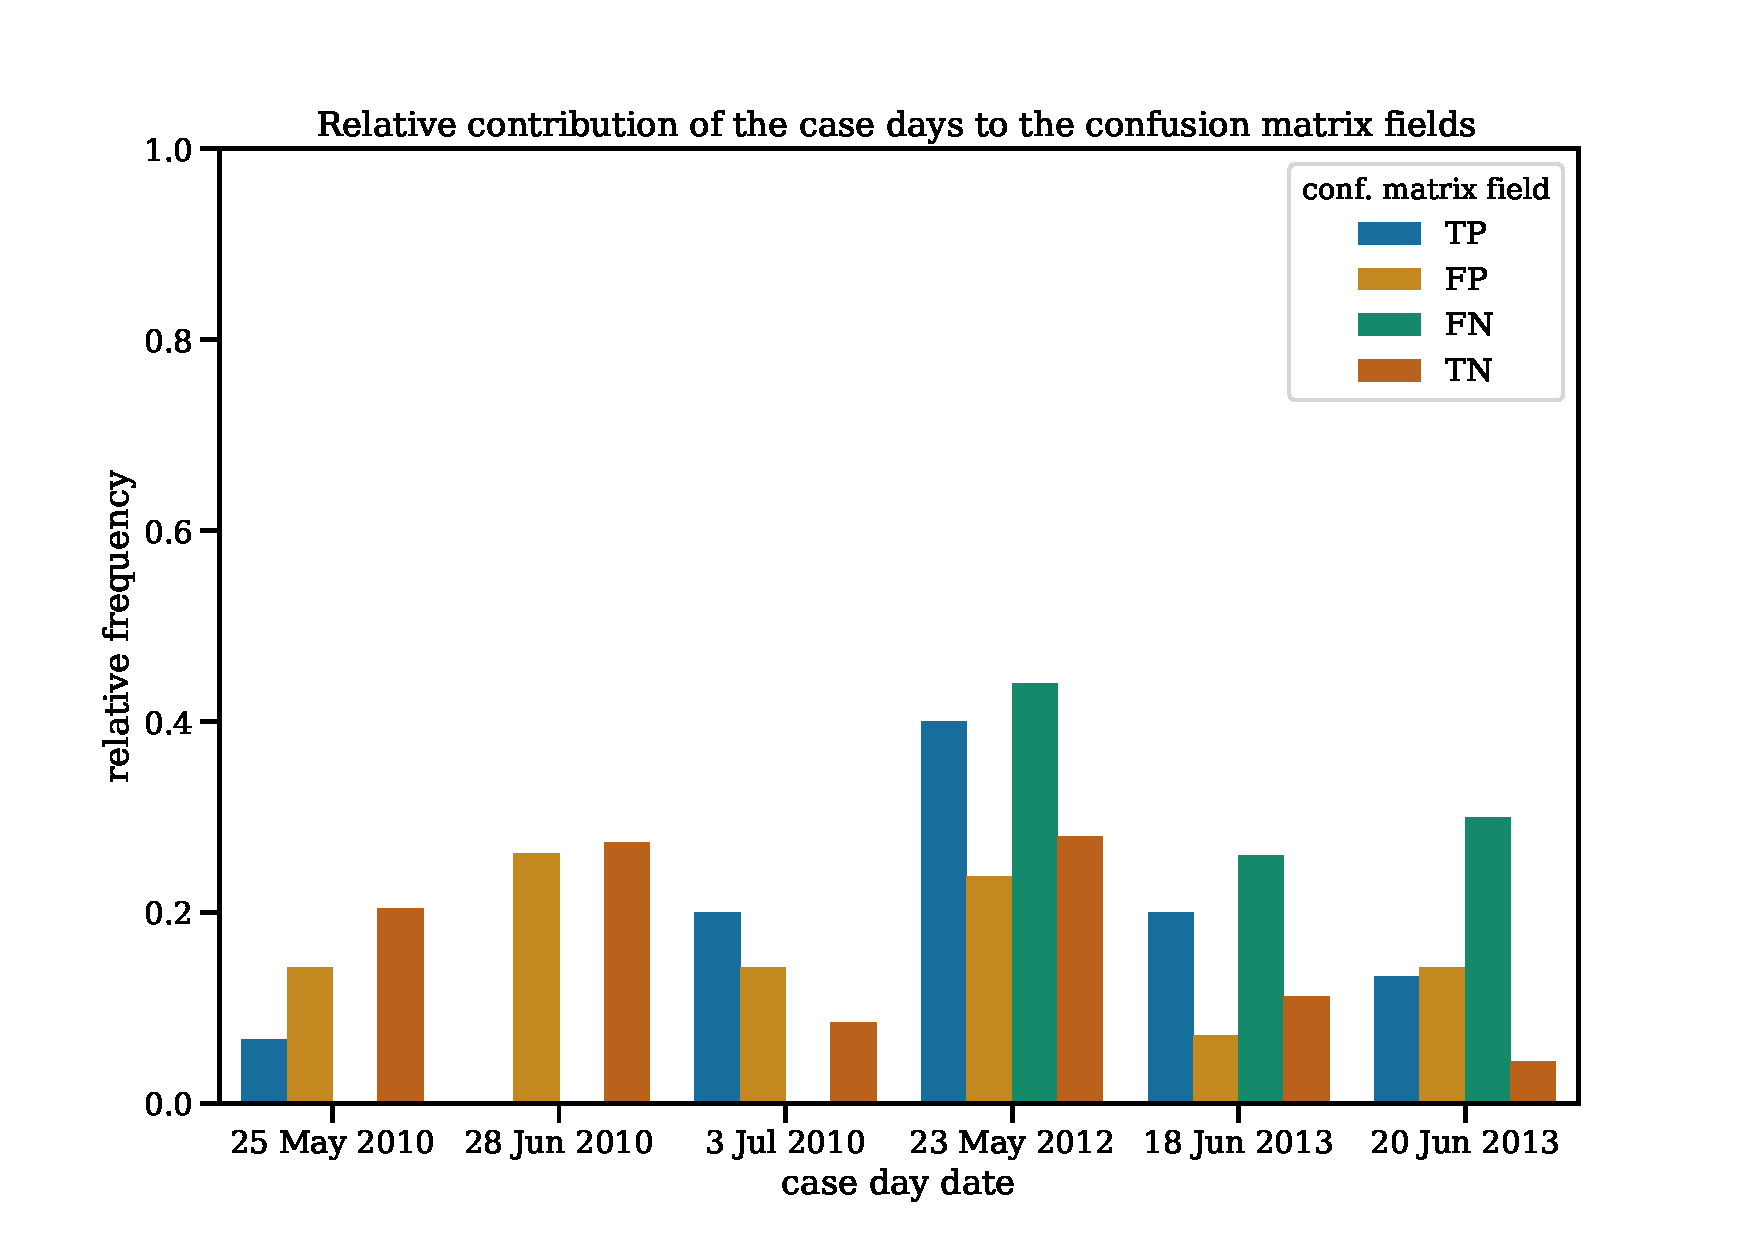
\includegraphics[width=0.8\textwidth]{Grafiken/Abbildungen/validation_case_day_frequencies.pdf}
\caption{Contribution of case days to the fields of the confusion matrix. Given is the relative proportion of cases per case day contributing to true positives (TP, blue), false positives (FP, yellow),false negatives (FN, green) and true negatives (TN, orange).}
\label{fig:validation_case_days}
\end{figure}


\begin{figure}[htbp]
\centering
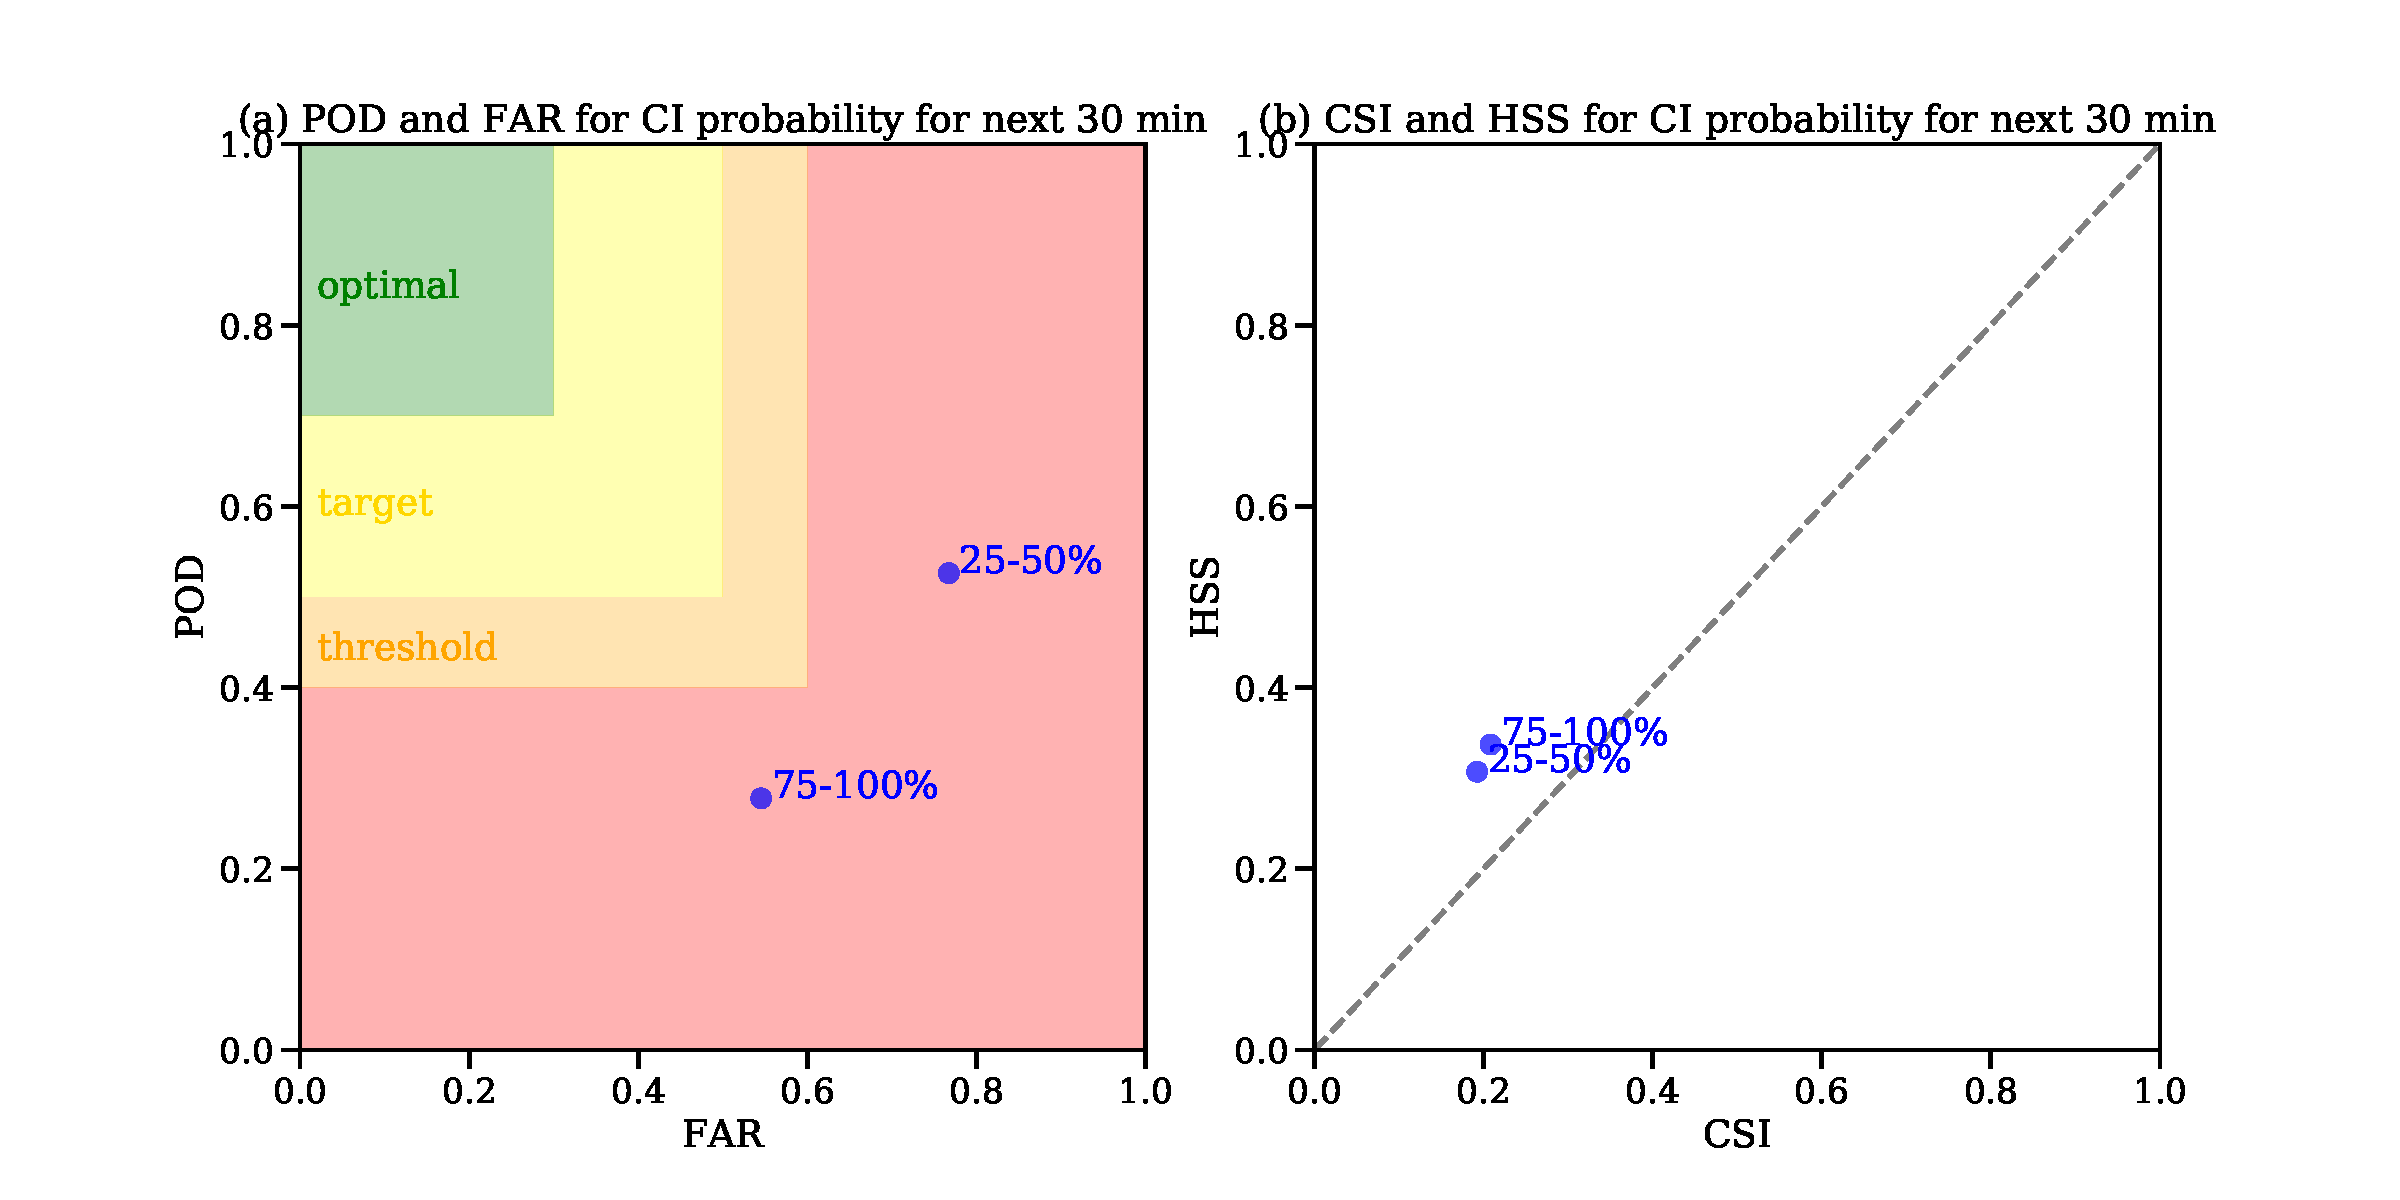
\includegraphics[width=\textwidth]{Grafiken/Abbildungen/validation_far_pod_hss_csi_plot.pdf}
\caption{Plot of the POD and FAR  and CSI and HSS of the validation of the CI product for the different CI probability levels. The colour surfaces in (a) denote the levels of POD and FAR given by the EUMETSAT requirements.}
\label{fig:validation_result2}
\end{figure}




